\begin{figure}[htpb!]
\centering
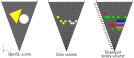
\includegraphics[width=\columnwidth]{images/volumetric/binary_decomposition}
\caption[Volumetric NED: Fixed pipeline decomposition]{Diagram shows the stages of our rendering pipeline: voxelization (see Section~\ref{sec:volumetric:Voxelization}) and binary decomposition (see Section~\ref{sec:volumetric:fixed_pipeline}). For ease of representation, the figure depicts the rendering pipeline for a simple 2-D graphics and 6 bits-per-pixel imagery. Actual implementation uses 3-D graphics and 24 bits-per-pixel imagery. The numbers along the displayed binary volume's frustum indicate the intensity level and color of the RGB LED that illuminates the current binary image.}
\label{fig:volumetric:binary_decomposition}
\end{figure}

